% =====================================================================
%  TAREA FINAL NOSQL - TEMPORADA ATP 2025
%  Compilar con pdfLaTeX
% =====================================================================
\documentclass[12pt]{article}

% ---------------------------------------------------------------------
%  DATOS DE LA PORTADA
% ---------------------------------------------------------------------
\newcommand{\autor}{Hugo Lucendo Romero}
\newcommand{\asignatura}{BASES DE DATOS NOSQL}
\newcommand{\fechaentrega}{05/11/2026}
\newcommand{\preguntaanalisis}{¿Fue la temporada 2025 cosa de dos jugadores?}

% ---------------------------------------------------------------------
%  PAQUETES (mismo estilo que el TFG)
% ---------------------------------------------------------------------
\usepackage[spanish, es-tabla]{babel}
\usepackage[utf8]{inputenc}
\usepackage[T1]{fontenc}
\usepackage[margin=3cm, top=3.4cm, headheight=1.4cm, headsep=0.7cm]{geometry}
\usepackage[skip=10pt plus1pt, indent=0pt]{parskip}
\usepackage{graphicx}
\usepackage[hidelinks]{hyperref}
\usepackage{booktabs}
\usepackage{float}
\usepackage{array}
\usepackage{tabularx}
\usepackage{xcolor}
\usepackage{fancyhdr}
\usepackage{caption}
\usepackage{listings}
\usepackage[most]{tcolorbox}

\graphicspath{{img/}}
\captionsetup{font=small, labelfont=bf, skip=6pt}
\setlength{\intextsep}{8pt plus 2pt minus 2pt}

% ---------------------------------------------------------------------
%  CABECERA Y PIE
% ---------------------------------------------------------------------
\pagestyle{fancy}
\fancyhf{}
\renewcommand{\headrulewidth}{0.4pt}
\fancyhead[L]{\small Hugo Lucendo Romero}
\fancyhead[R]{
\includegraphics[height=1.05cm]{ucm}}
\fancyhead[C]{\small Tarea Final NoSQL -- Temporada ATP 2025}
\fancyfoot[C]{\thepage}

\fancypagestyle{portada}{%
  \fancyhf{}
  \renewcommand{\headrulewidth}{0pt}
  \fancyhead[R]{
\includegraphics[height=1.05cm]{ucm}}
}

% ---------------------------------------------------------------------
%  APARTADOS CON NUMERACIÓN PROPIA
% ---------------------------------------------------------------------
\newcommand{\seccion}[2]{%
  \section*{#1\quad #2}\addcontentsline{toc}{section}{\protect\numberline{#1}#2}}
\newcommand{\subseccion}[2]{%
  \subsection*{#1\quad #2}\addcontentsline{toc}{subsection}{\protect\numberline{#1}#2}}
\newcommand{\pregunta}[2]{%
  \subsection*{#1.\quad #2}\addcontentsline{toc}{subsection}{\protect\numberline{#1}#2}}

% ---------------------------------------------------------------------
%  ESTILO DEL CÓDIGO (consola de MongoDB y Python)
% ---------------------------------------------------------------------
\definecolor{codkey}{HTML}{1F3F7A}
\definecolor{codstr}{HTML}{8B2A1A}
\definecolor{codcom}{HTML}{4F7A3C}

\lstdefinelanguage{mongo}{
  morekeywords={var, use, db, true, false, null},
  sensitive=true,
  morecomment=[l]{//},
  morestring=[b]"
}

\lstdefinestyle{mongosh}{
  language=mongo,
  basicstyle=\ttfamily\footnotesize,
  keywordstyle=\color{codkey}\bfseries,
  stringstyle=\color{codstr},
  commentstyle=\color{codcom}\itshape,
  showstringspaces=false,
  breaklines=true,
  breakatwhitespace=true,
  columns=fullflexible,
  keepspaces=true,
  tabsize=4,
  upquote=true,
  aboveskip=0pt, belowskip=0pt
}

\lstdefinestyle{python}{
  language=Python,
  basicstyle=\ttfamily\footnotesize,
  keywordstyle=\color{codkey}\bfseries,
  stringstyle=\color{codstr},
  commentstyle=\color{codcom}\itshape,
  showstringspaces=false,
  breaklines=true,
  breakatwhitespace=true,
  columns=fullflexible,
  keepspaces=true,
  tabsize=4,
  upquote=true,
  aboveskip=0pt, belowskip=0pt
}

% Bloque de código: lo único que va en recuadro
\tcbset{
  codigo/.style={enhanced, unbreakable, colback=black!3, colframe=black!35,
                 boxrule=0.4pt, arc=0pt, left=4pt, right=4pt, top=3pt, bottom=3pt,
                 before skip=6pt, after skip=8pt},
  codigolargo/.style={codigo, breakable}
}
\newcommand{\consulta}[1]{%
  \tcbinputlisting{codigo, listing only, listing file=js/#1.js,
                   listing options={style=mongosh}}}
\newcommand{\codigopython}[1]{%
  \tcbinputlisting{codigolargo, listing only, listing file=py/#1.py,
                   listing options={style=python}}}

% Rótulos ("Consulta", "Resultado", "Interpretación")
\newcommand{\rotulo}[1]{\par\textbf{#1}\par\nobreak\vspace{-4pt}}

% Captura del resultado con pie numerado
%   #1 archivo (sin .png)   #2 pie de tabla
\newcommand{\resultado}[2]{%
  \IfFileExists{img/#1.png}{%
    \begin{table}[H]
      \centering
      \vspace{6pt}
      \rule{\linewidth}{0.8pt}\\[3pt]
      \includegraphics[width=\linewidth,height=0.30\textheight,keepaspectratio]{#1}\\[-1pt]
      \rule{\linewidth}{0.8pt}
      \caption{#2}
    \end{table}}{%
    \begin{table}[H]
      \centering
      \fbox{\parbox{0.9\linewidth}{\centering\small\vspace{1cm}
        Captura pendiente: \texttt{\detokenize{img/#1.png}}\vspace{1cm}}}
      \caption{#2}
    \end{table}}}

% Captura adicional (sin pie) solo si existe el archivo
\newcommand{\resultadoextra}[1]{%
  \IfFileExists{img/#1.png}{%
    \begin{center}\vspace{-4pt}
      \includegraphics[width=\linewidth,height=0.30\textheight,keepaspectratio]{#1}\\[-1pt]
      \rule{\linewidth}{0.8pt}
    \end{center}}{}}

% Dos capturas en fila con un solo pie
%   #1 y #2 archivos (sin .png)   #3 pie de tabla
\newcommand{\resultadodoble}[3]{%
  \begin{table}[H]
    \centering
    \vspace{6pt}
    \rule{\linewidth}{0.8pt}\\[3pt]
    \begin{minipage}[t]{0.49\linewidth}\vspace{0pt}
      \includegraphics[width=\linewidth]{#1}
    \end{minipage}\hfill
    \begin{minipage}[t]{0.49\linewidth}\vspace{0pt}
      \includegraphics[width=\linewidth]{#2}
    \end{minipage}\\[-1pt]
    \rule{\linewidth}{0.8pt}
    \caption{#3}
  \end{table}}

% Gráfica del notebook con pie numerado
\newcommand{\grafica}[2]{%
  \begin{figure}[H]
    \centering
    \includegraphics[width=0.65\linewidth]{#1}
    \caption{#2}
  \end{figure}}

% =====================================================================
\begin{document}
% =====================================================================

% ---------------------------------------------------------------------
%  PORTADA
% ---------------------------------------------------------------------
\thispagestyle{portada}
\begin{center}
  \vspace*{1cm}
  {\huge\bfseries TAREA FINAL NOSQL -- TEMPORADA ATP 2025\par}
  \vspace{0.3cm}
  {\large Análisis de los partidos del circuito ATP con MongoDB\par}
  \vspace{0.9cm}
  \IfFileExists{img/portada.png}{\includegraphics[width=0.6\textwidth]{portada}}{}
\end{center}
\vfill
\begin{flushright}
  \large\bfseries
  \autor\\[0.9em]
  \asignatura\\[0.9em]
  \fechaentrega
\end{flushright}

% ---------------------------------------------------------------------
%  ÍNDICE
% ---------------------------------------------------------------------
\newpage
\tableofcontents

% ---------------------------------------------------------------------
%  1. INTRODUCCIÓN
% ---------------------------------------------------------------------
\newpage
\seccion{1}{Introducción}

Este documento presenta el análisis de la temporada 2025 del circuito ATP mediante una base de datos MongoDB. El trabajo incluye la carga del dataset, consultas de inserción, actualización, proyección y filtrado, consultas con el pipeline de agregación y, como parte adicional, la conexión a la base de datos desde Python para representar algunos de los resultados en gráficas.

El análisis gira en torno a una pregunta:

\begin{center}
  \textit{\preguntaanalisis}
\end{center}

En 2025 Carlos Alcaraz y Jannik Sinner se repartieron los cuatro Grand Slam, pero eso no significa por sí solo que el resto de jugadores no tuviera peso en la temporada. Por ello, además de comparar a ambos con el resto del circuito, se estudia cómo influyen en los partidos factores como la superficie, el número de sets o la altura de los jugadores, y hasta qué punto el ranking anticipa al ganador.

Cada consulta se presenta en el orden consulta, resultado e interpretación. Todas las consultas se encuentran también en el script \texttt{consultas\_tenis.js} que se entrega junto a este documento, de forma que se pueden ejecutar en el mismo orden.

% ---------------------------------------------------------------------
%  2. DATASET
% ---------------------------------------------------------------------
\bigskip
\seccion{2}{Dataset}
\subseccion{2.1}{Origen de los datos}

Los datos proceden de TML-Database (\url{https://github.com/Tennismylife/TML-Database}), un repositorio público que recoge todos los partidos del circuito ATP a partir de la información oficial de la ATP y que sigue el mismo formato que la conocida base de datos de Jeff Sackmann. Se ha utilizado el fichero de la temporada 2025, que contiene 2944 partidos jugados en 197 torneos entre el 29/12/2024 y el 22/12/2025, incluyendo Grand Slam, Masters 1000, ATP 500, ATP 250, ATP Finals, Copa Davis y otras competiciones como la United Cup, la Laver Cup o las Next Gen ATP Finals.

\subseccion{2.2}{Transformación de CSV a JSON}

El fichero original es un CSV en el que cada partido ocupa una fila con 49 columnas: unas describen el torneo y el partido, y el resto se repiten dos veces, una para el ganador (\texttt{winner\_*}, \texttt{w\_*}) y otra para el perdedor (\texttt{loser\_*}, \texttt{l\_*}). Importarlo tal cual en MongoDB daría documentos planos, equivalentes a una tabla relacional, y no se aprovecharía el modelo de documentos.

Por ello, antes de la carga se ha escrito un script en Python (\texttt{convertir\_csv\_a\_json.py}, que se entrega junto al resto de ficheros) que convierte cada fila en un documento siguiendo el modelo embebido. Los datos del ganador y del perdedor se agrupan en dos documentos embebidos, \texttt{ganador} y \texttt{perdedor}, ya que tienen una relación 1-1 con el partido y siempre se consultan junto a él, y sus estadísticas de saque se agrupan a su vez en un documento \texttt{estadisticas}. Además, el resultado, que en el CSV es un texto como \texttt{4-6 6-7(4) 6-4 7-6(3) 7-6(2)}, se separa en un array \texttt{sets} con un documento por cada set jugado, lo que permite consultar los sets de forma individual.

Durante la conversión se han tenido en cuenta varios casos particulares del dataset:

\begin{itemize}
  \item Los valores vacíos del CSV se guardan como \texttt{null} y los números se convierten a entero o decimal.
  \item La fecha se transforma del formato \texttt{20250526} a \texttt{2025-05-26}, para poder convertirla después a tipo fecha con \texttt{\$toDate}.
  \item En los sets con tiebreak el CSV solo indica los puntos de quien lo pierde, por ejemplo \texttt{7-6(4)}. Los puntos de quien lo gana se calculan como 7 o dos más que el rival, salvo en el quinto set de los Grand Slam, donde el tiebreak se juega a 10 puntos.
  \item En la Copa Davis y la Laver Cup el tercer set se sustituye por un súper tiebreak a 10 puntos (\texttt{[10-8]}), que se guarda como un set sin juegos y solo con los puntos del tiebreak.
  \item Las retiradas (\texttt{RET}) y los partidos no disputados (\texttt{W/O}) se identifican en un campo \texttt{final}.
  \item La última fila del CSV venía incompleta a mitad de las estadísticas (la final de las Next Gen ATP Finals). El resto de datos del partido es correcto, por lo que se ha mantenido el partido dejando sus estadísticas vacías.
\end{itemize}

\subseccion{2.3}{Estructura de los documentos}

Cada documento de la colección \texttt{partidos} representa un partido. En la Tabla \ref{tab:campos} se describen los campos más relevantes para el análisis.

\begin{table}[H]
  \centering
  \footnotesize
  \begin{tabularx}{\textwidth}{@{} l l X @{}}
    \toprule
    \textbf{Campo} & \textbf{Tipo} & \textbf{Descripción} \\
    \midrule
    \texttt{torneo} & String & Nombre del torneo \\
    \texttt{superficie} & String & Superficie de la pista: pista dura, tierra batida o hierba \\
    \texttt{nivel} & String & Categoría del torneo (G Grand Slam, M Masters 1000, 500, 250, F ATP Finals, D Copa Davis, A otros) \\
    \texttt{fecha} & String & Fecha de inicio del torneo (no del partido) \\
    \texttt{ronda} & String & Ronda del partido (R128 \ldots{} F, RR en fases de grupos) \\
    \texttt{al\_mejor\_de} & Int & Número máximo de sets del partido (3 o 5) \\
    \texttt{resultado} & String & Resultado original del CSV \\
    \texttt{sets} & Array & Un documento por set: \texttt{juegos\_ganador}, \texttt{juegos\_perdedor} y \texttt{tiebreak} \\
    \texttt{final} & String & Cómo termina el partido: completo, retirada o walkover \\
    \texttt{minutos} & Int & Duración del partido \\
    \texttt{ganador} / \texttt{perdedor} & Object & Nombre, país, mano, altura, edad, ranking, puntos de ranking y estadísticas \\
    \texttt{\ldots estadisticas} & Object & Aces, dobles faltas, puntos y juegos al saque, primeros saques y bolas de break \\
    \bottomrule
  \end{tabularx}
  \caption{Campos principales de la colección \texttt{partidos}}
  \label{tab:campos}
\end{table}

Hay que tener en cuenta que el ranking de cada jugador es el que tenía en la semana de inicio del torneo, por lo que es el mismo en todas las rondas, y que la fecha corresponde también al inicio del torneo y no al día del partido.

\subseccion{2.4}{Carga en MongoDB}

El fichero \texttt{atp\_partidos\_2025.json} se ha importado con MongoDB Compass en la base de datos \texttt{tenis-2025}, dentro de la colección \texttt{partidos}.

\resultado{carga_2}{Colección \texttt{partidos} después de la importación}

La importación carga los 2944 partidos. A continuación se comprueba el número de documentos y la estructura de uno de ellos desde la consola.

\rotulo{Consulta}
\consulta{crud_1}

\rotulo{Resultado}
\resultado{crud_1}{Número de documentos y estructura de un partido}

% ---------------------------------------------------------------------
%  3. INSERCIÓN, ACTUALIZACIÓN, PROYECCIÓN Y FILTRADO
% ---------------------------------------------------------------------
\newpage
\seccion{3}{Inserción, Actualización, Proyección y Filtrado}

\pregunta{3.1}{Traducción de las superficies}

Las superficies vienen en inglés (Hard, Clay y Grass). Para que los resultados se lean mejor, se traducen al castellano con un \texttt{updateMany} por cada superficie.

\rotulo{Consulta}
\consulta{crud_2}

\rotulo{Resultado}
\resultado{crud_2}{Superficies antes y después de la actualización}

\rotulo{Interpretación}

Se modifican 1860 partidos de pista dura, 787 de tierra y 297 de hierba, que suman los 2944 partidos de la colección. Ya se ve desde el principio que la temporada se juega sobre todo en pista dura, casi dos de cada tres partidos, mientras que la hierba apenas supone un 10\%.

\bigskip
\pregunta{3.2}{Partidos con y sin estadísticas}

No todos los partidos tienen estadísticas de saque. Como en los datos todas las estadísticas aparecen o faltan a la vez, basta con comprobar los aces del ganador. Se añade un campo \texttt{con\_estadisticas} para poder filtrar después estos partidos.

\rotulo{Consulta}
\consulta{crud_3}

\rotulo{Resultado}
\resultado{crud_3}{Partidos marcados con y sin estadísticas}

\rotulo{Interpretación}

193 partidos no tienen estadísticas, un 6.6\% del total, y los 2751 restantes sí. La segunda actualización usa \texttt{\$exists: false}, ya que después de la primera los únicos documentos que no tienen el campo son justo los que tienen estadísticas. Todas las consultas posteriores sobre aces o saque se harán sobre los partidos con \texttt{con\_estadisticas: true}.

\bigskip
\pregunta{3.3}{Colección de niveles de torneo}

El campo \texttt{nivel} guarda un código que no se entiende por sí solo. Se crea una segunda colección, \texttt{niveles}, con el nombre de cada nivel y los puntos que se lleva el campeón, que se utilizará más adelante en una agregación.

\rotulo{Consulta}
\consulta{crud_4}

\rotulo{Resultado}
\resultado{crud_4}{Inserción de la colección \texttt{niveles}}

\rotulo{Interpretación}

Se insertan los 7 niveles. La Copa Davis y el grupo de otras competiciones no tienen el campo \texttt{puntos\_campeon}, ya que no reparten puntos fijos por ganar el torneo, y MongoDB permite guardarlos igualmente sin ese campo, al no exigir que todos los documentos de una colección tengan la misma estructura.

\bigskip
\pregunta{3.4}{Inserción, modificación y borrado de un partido}

Para probar las operaciones sobre un único documento se inserta el primer partido de la temporada 2026, solo con algunos campos, se completa con su duración y sus sets y, como el análisis es de 2025, se borra al final.

\rotulo{Consulta}
\consulta{crud_5}

\rotulo{Resultado}
\resultadodoble{crud_5}{crud_5_c}{Inserción, actualización y borrado de un partido de 2026}

\rotulo{Interpretación}

El partido se inserta con menos campos que el resto, sin estadísticas ni sets. Con \texttt{\$set} se añade el campo \texttt{minutos}, que no existía, y con \texttt{\$push} y \texttt{\$each} se crea el array \texttt{sets} con los dos sets a la vez. Tras el \texttt{deleteOne} la colección vuelve a tener 2944 partidos.

\bigskip
\pregunta{3.5}{Finales de los Grand Slam}

\rotulo{Consulta}
\consulta{crud_6}

\rotulo{Resultado}
\resultado{crud_6}{Finales de los cuatro Grand Slam de 2025}

\rotulo{Interpretación}

Sinner gana el Open de Australia y Wimbledon, y Alcaraz Roland Garros y el US Open, por lo que entre los dos se reparten los cuatro grandes. Además, tres de las cuatro finales las juegan entre ellos, y solo Zverev consigue colarse en la de Australia.

Llama la atención la duración de la final de Roland Garros, 329 minutos, el doble que las otras tres (entre 162 y 184 minutos). Alcaraz la gana remontando dos sets en contra, y el quinto set se decide en un tiebreak a 10 puntos.

\bigskip
\pregunta{3.6}{Partidos entre Alcaraz y Sinner}

\rotulo{Consulta}
\consulta{crud_7}

\rotulo{Resultado}
\resultadodoble{crud_7}{crud_7_b}{Partidos entre Alcaraz y Sinner en 2025}

\rotulo{Interpretación}

Se enfrentan seis veces y todas en una final, en Roma, Roland Garros, Wimbledon, Cincinnati, el US Open y las ATP Finals, es decir, en las tres superficies. Alcaraz gana cuatro y Sinner dos, aunque una de las victorias de Alcaraz, la de Cincinnati, llega por retirada de Sinner con 5-0 en el primer set, por lo que en partidos completos el balance es más ajustado de lo que indica el 4-2.

\bigskip
\pregunta{3.7}{Partidos más largos de la temporada}

\rotulo{Consulta}
\consulta{crud_8}

\rotulo{Resultado}
\resultadodoble{crud_8}{crud_8_b}{Los 5 partidos más largos de 2025}

\rotulo{Interpretación}

Los cinco son de Grand Slam y se van al quinto set, lo cual es lógico porque es el único torneo en el que se juega al mejor de cinco sets. Sin embargo, salvo la final de Roland Garros, todos son de primeras rondas, y todos tienen al menos dos tiebreaks. Los partidos más largos no salen de muchos juegos, sino de sets muy igualados.

\bigskip
\pregunta{3.8}{Consultas sobre el array de sets}

En esta consulta se cuentan primero los partidos que llegan al quinto set y después los partidos ganados por un jugador que perdió algún set 6-7, comparando el resultado con y sin \texttt{\$elemMatch}.

\rotulo{Consulta}
\consulta{crud_9}

\rotulo{Resultado}
\resultado{crud_9}{Partidos a cinco sets y comparación con y sin \texttt{\$elemMatch}}

\rotulo{Interpretación}

101 partidos llegan al quinto set. En la segunda parte, sin \texttt{\$elemMatch} salen 381 partidos y con \texttt{\$elemMatch} 281. La diferencia se debe a que, sin \texttt{\$elemMatch}, cada condición se puede cumplir en un set distinto: un partido como \texttt{6-4 5-7 6-3} cuenta, porque tiene un set con 6 juegos del ganador y otro con 7 del perdedor, aunque ningún set acabe 6-7. Con \texttt{\$elemMatch} las dos condiciones se tienen que cumplir en el mismo set, que es lo que se busca, por lo que 100 de los partidos de la primera consulta son falsos positivos.

% ---------------------------------------------------------------------
%  4. PIPELINE DE AGREGACIÓN
% ---------------------------------------------------------------------
\newpage
\seccion{4}{Pipeline de Agregación}

\pregunta{4.1}{Partidos y duración media por superficie}

\rotulo{Consulta}
\consulta{agg_1}

\rotulo{Resultado}
\resultado{agg_1}{Partidos y duración media por superficie}

\rotulo{Interpretación}

Los partidos en hierba son los más largos, con 130 minutos de media, frente a 115 en pista dura y 109 en tierra. El resultado es curioso, porque la hierba es la superficie más rápida y se esperaría que los puntos y los partidos fueran más cortos, así que en la siguiente consulta se separan los partidos según el número de sets.

\bigskip
\pregunta{4.2}{Duración media por superficie y número de sets}

\rotulo{Consulta}
\consulta{agg_2}

\rotulo{Resultado}
\resultadodoble{agg_2}{agg_2_b}{Duración media por superficie y número máximo de sets}

\rotulo{Interpretación}

Al comparar partidos iguales, al mejor de tres sets, la hierba pasa a ser la superficie con los partidos más cortos (106.9 minutos), aunque las tres están muy cerca. La media anterior salía más alta porque 127 de los 297 partidos en hierba son de Wimbledon, al mejor de cinco sets, mientras que en pista dura esa proporción es mucho menor.

Por otro lado, en tierra solo aparece un partido al mejor de cinco sets, cuando Roland Garros tiene 127. Revisando los datos, Roland Garros es el torneo con más partidos sin duración: solo la tiene la final. Por tanto, la media de la tierra no incluye los partidos largos de Roland Garros y hay que tomarla con cuidado.

\bigskip
\pregunta{4.3}{Títulos y puntos por jugador}

En esta consulta se une cada final con la colección \texttt{niveles} mediante \texttt{\$lookup} para saber cuántos puntos da cada título.

\rotulo{Consulta}
\consulta{agg_3}

\rotulo{Resultado}
\resultadodoble{agg_3}{agg_3_b}{Jugadores con más puntos por títulos}

\rotulo{Interpretación}

Alcaraz gana 8 títulos que suman 8500 puntos y Sinner 6 que suman 7500. Entre los dos acumulan 16000 puntos solo en títulos, frente a los 3500 que suman los tres siguientes juntos. Alcaraz gana más torneos y en las tres superficies, mientras que Sinner gana menos, pero casi todos son de los más importantes.

El caso de Bublik muestra la diferencia entre ganar muchos títulos y ganar títulos importantes, ya que con 4 títulos suma los mismos puntos que Ruud con 2. En el quinto puesto aparece Valentin Vacherot, que gana el Masters 1000 de Shanghái siendo el número 202 del mundo.

Los puntos están simplificados, ya que solo se cuentan los que da ganar el torneo y no los de cada ronda, pero sirven para comparar el peso de los títulos de cada jugador.

\bigskip
\pregunta{4.4}{Balance de victorias de todos los jugadores}

Para calcular los partidos jugados por cada jugador hay que tener en cuenta que aparece unas veces como ganador y otras como perdedor. Por eso, cada partido se transforma en un array con los dos jugadores y se separa con \texttt{\$unwind}. El resultado se guarda con \texttt{\$out} en una colección nueva, \texttt{jugadores}, para no tener que volver a calcularlo.

\rotulo{Consulta}
\consulta{agg_4}

\rotulo{Resultado}
\resultado{agg_4}{Creación de la colección \texttt{jugadores} con \texttt{\$out}}

Una vez guardada, se consulta directamente la colección \texttt{jugadores} para obtener los mejores porcentajes de victoria entre los jugadores con al menos 40 partidos.

\rotulo{Consulta}
\consulta{agg_4b}

\rotulo{Resultado}
\resultadodoble{agg_4_b}{agg_4_c}{Mejores porcentajes de victoria con al menos 40 partidos}

\rotulo{Interpretación}

La colección \texttt{jugadores} tiene 455 jugadores distintos. Sinner es el jugador con mejor porcentaje de victorias (90.6\%) por delante de Alcaraz (88.75\%), aunque Alcaraz gana más partidos, 71 frente a 58, porque juega 16 partidos más. Esto se explica porque Sinner no juega entre febrero y abril, como se ve en la consulta 4.7.

Detrás de ellos hay un salto de más de diez puntos hasta Djokovic (78\%), que juega pocos torneos pero los aprovecha. Zverev, que gana tantos partidos como Sinner, se queda en un 69.9\% porque necesita 83 partidos para conseguirlo.

\bigskip
\pregunta{4.5}{Porcentaje de sets que acaban en tiebreak por superficie}

\rotulo{Consulta}
\consulta{agg_5}

\rotulo{Resultado}
\resultado{agg_5}{Sets y tiebreaks por superficie}

\rotulo{Interpretación}

En hierba el 22.2\% de los sets acaba en tiebreak, frente al 19.5\% en pista dura y el 14.7\% en tierra. En la hierba el saque tiene más ventaja y es más difícil romperlo, por lo que los sets llegan más veces al 6-6, mientras que en tierra hay más breaks y los sets se deciden antes. Los súper tiebreaks de la Copa Davis se excluyen con el \texttt{\$match}, ya que no son sets con juegos.

\bigskip
\pregunta{4.6}{Aces según la altura del jugador}

En esta consulta se agrupan los jugadores por tramos de altura con \texttt{\$bucket} y se calcula la media de aces por partido en cada tramo.

\rotulo{Consulta}
\consulta{agg_6}

\rotulo{Resultado}
\resultado{agg_6_b}{Media de aces por partido según la altura}

\rotulo{Interpretación}

La media de aces aumenta en todos los tramos, desde 2.2 aces por partido en los jugadores de menos de 1.75 metros hasta 12.4 en los de más de 2 metros, casi seis veces más. La altura permite sacar desde más arriba y con un ángulo mejor, y los datos lo reflejan de forma muy clara. El tramo con más partidos es el de 1.85 a 1.89 metros, que es la altura más habitual en el circuito.

\bigskip
\pregunta{4.7}{Victorias de Alcaraz y Sinner por mes}

\rotulo{Consulta}
\consulta{agg_7}

\rotulo{Resultado}
\resultadodoble{agg_7}{agg_7_c}{Victorias de Alcaraz y Sinner por mes}

\rotulo{Interpretación}

Sinner no tiene victorias en febrero, marzo ni abril, ya que en 2025 cumplió una sanción de tres meses, y vuelve en mayo directamente con 11 victorias. Durante esos meses Alcaraz suma 20 victorias, lo que explica buena parte de su diferencia de partidos ganados en la temporada.

Ninguno de los dos tiene victorias en julio, aunque Sinner gana Wimbledon. Esto se debe a que la fecha de los partidos es la de inicio del torneo y Wimbledon empezó el 30 de junio, por lo que todas sus victorias cuentan en junio. También destaca octubre, en el que Sinner suma 10 victorias y Alcaraz ninguna.

% ---------------------------------------------------------------------
%  5. VISUALIZACIÓN CON PYTHON
% ---------------------------------------------------------------------
\bigskip
\seccion{5}{Visualización con Python}

Como parte adicional, en el notebook \texttt{graficas\_tenis.ipynb} se conecta a la base de datos desde Python con la librería pymongo, se lanzan algunas de las agregaciones anteriores y se representan con matplotlib. Las agregaciones son las mismas que en la consola, cambiando solo las claves, que van entre comillas, y \texttt{null} por \texttt{None}.

\codigopython{conexion}

En el caso de las victorias por mes, los meses sin victorias no aparecen en el resultado de la agregación, por lo que se crean dos listas de 12 meses a cero y se rellenan con los resultados.

\codigopython{meses}

\grafica{victorias_mes}{Victorias de Alcaraz y Sinner por mes en 2025}

En la gráfica se ve claramente el periodo sin jugar de Sinner y que, en los meses en los que juegan los dos, sus victorias son muy parecidas, salvo en octubre.

\grafica{top10_porcentaje}{Top 10 en porcentaje de victorias (mínimo 40 partidos)}

Esta gráfica se obtiene directamente de la colección \texttt{jugadores} guardada con \texttt{\$out}, sin repetir la agregación, y muestra la distancia entre Sinner y Alcaraz y el resto de jugadores.

\begin{figure}[H]
  \centering
  \begin{minipage}{0.48\linewidth}
    \centering
    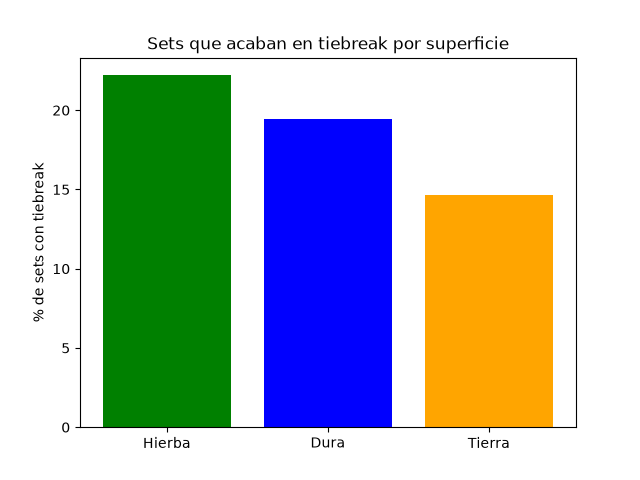
\includegraphics[width=\linewidth]{tiebreaks_superficie}
    \caption{Sets que acaban en tiebreak por superficie}
  \end{minipage}\hfill
  \begin{minipage}{0.48\linewidth}
    \centering
    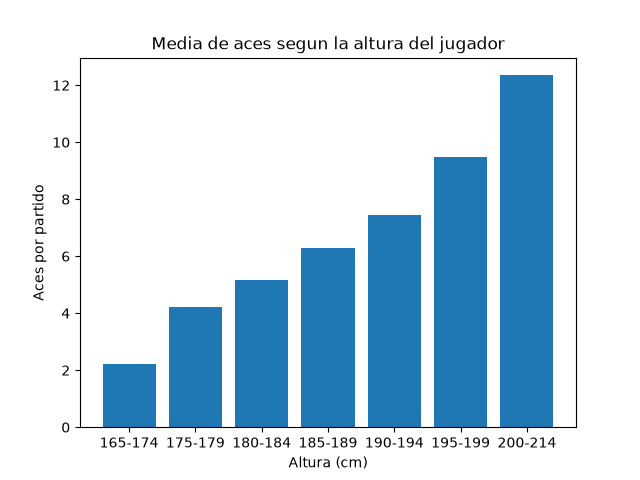
\includegraphics[width=\linewidth]{aces_altura}
    \caption{Aces por partido según la altura}
  \end{minipage}
\end{figure}

En las dos últimas gráficas se ve el peso del saque según la superficie y según la altura del jugador, con una relación creciente en ambos casos.

% ---------------------------------------------------------------------
%  6. CONCLUSIONES
% ---------------------------------------------------------------------
\newpage
\seccion{6}{Conclusiones}

Volviendo a la pregunta inicial, los datos indican que la temporada 2025 sí fue en gran medida cosa de dos jugadores. Alcaraz y Sinner se reparten los cuatro Grand Slam, juegan seis finales entre ellos, son los únicos con más de 40 partidos que superan el 80\% de victorias y acumulan más del cuádruple de puntos en títulos que los tres siguientes juntos. Entre ellos la temporada está muy igualada: Alcaraz gana más partidos y más títulos, pero Sinner tiene mejor porcentaje de victorias pese a estar tres meses sin competir.

Por debajo de ellos, el ranking no siempre anticipa al ganador. Jugadores como Vacherot, que gana un Masters 1000 siendo el número 202, muestran que el resto del circuito también tiene margen para dar sorpresas.

En cuanto al juego, la superficie condiciona el desarrollo de los partidos. En hierba hay más tiebreaks y en tierra menos, lo que refleja la ventaja del saque en las superficies rápidas, y esa ventaja aumenta con la altura del jugador. En cambio, la duración de los partidos depende sobre todo del número de sets y no de la superficie, y la diferencia que aparece a primera vista en la hierba se debe al peso de Wimbledon.

Por último, hay que tener en cuenta las limitaciones del dataset: faltan la duración de casi todo Roland Garros y las estadísticas de 193 partidos, y tanto el ranking como la fecha corresponden a la semana de inicio de cada torneo, lo que hay que tener presente al interpretar los resultados por mes o por ranking.

\end{document}
